\section{Experimental Results}\label{sec:evaluation}

\subsection{Speculation profitability and training cost}\label{sec:measure}

The calibration measurements (\cref{app:calibration}; Figure~\ref{fig:motivation}) show the three effects that make speculation and training one decision.

\paragraph{Whether speculation pays depends on load and architecture.} For Qwen3-8B with short outputs, speculation is \nv{sweep.short.c1}\% faster than plain decoding at $C{=}1$ but \nv{sweep.short.c256abs}\% slower at $C{=}256$ (Figure~\ref{fig:motivation}a); with long outputs it remains \nv{sweep.long.c96}\% faster at $C{=}96$. The MoE target behaves the other way: its gain grows to \nv{sweep.moe.c64}\% at $C{=}64$ and is still \nv{sweep.moe.c256}\% at $C{=}256$, because a speculative step costs only \nv{step.m2.c256}$\times$ a plain step there, against \nv{step.m1.c256}$\times$ on the dense target \citep{huang2025moesd}.

\paragraph{Co-located training is not free.} At duty cycle $d$ the trainer computes for a fraction $d$ of the time, and serving throughput falls almost linearly, by $\kappa(C)\,d$ with $\kappa$ between \nv{kappa.min} and \nv{kappa.max} (Figure~\ref{fig:motivation}b): duty 0.5 costs \nv{duty.d05.lossmin}--\nv{duty.d05.lossmax}\% of throughput, and training all the time costs \nv{duty.d10.lossmin}--\nv{duty.d10.lossmax}\%.

\paragraph{Learning ceilings differ, and the frontier is linear.} After learning online from $N$ requests (Figure~\ref{fig:motivation}c), the code and SQL drafters improve steadily, the Chinese drafter stalls at \nv{lc.zh.n3200} because only \nv{cover.zh}\% of the target's output tokens are in its 32k draft vocabulary, and the function-calling drafter peaks at $N{=}\nv{lc.fc.peakN}$ and then declines. Against the break-even line at $C{=}256$, the code drafter crosses after about 100 requests, the Chinese drafter never does, and the MoE drafter is above its much lower break-even (\nv{astar.moe.c256}) from the start. The throughput ratio of three or four drafter checkpoints at six loads is close to linear in acceptance at every load (Figure~\ref{fig:frontier}): the fit of \cref{eq:frontier} has residuals of at most \nv{astar.code.err} (code), \nv{astar.zh.err} (Chinese), and \nv{astar.moe.err} (MoE), and the adapted code drafter reaches \nv{fr.code.n3200.c256}$\times$ plain decoding there against \nv{fr.code.n0.c256}$\times$ for the factory drafter. Training is therefore worth doing only if the trained drafter will be used, which depends on load, and at saturation the drafter may become usable only after training.

\subsection{End-to-end serving performance}\label{sec:results}

\begin{table*}[t]
\caption{Phase-B (saturated) throughput relative to \pol{Static}: paired mean $\pm$ sd over three repetitions, \%. Parentheses: fraction of the best policy in the scenario (bold); \pol{Static} row: absolute throughput; last column: smallest fraction over the three scenarios.}
\label{tab:main}
\centering\small

% Generated table style: Main Results
\renewcommand{\arraystretch}{1.15}
\setlength{\tabcolsep}{4pt}

\begin{tabular}{@{}lcccc@{}}
\toprule
\textbf{Policy} &
\textbf{8B Code} &
\textbf{8B Chinese} &
\textbf{MoE Code} &
\textbf{Worst Case} \\
\midrule

% ===== Serving baselines =====
\rowcolor{tabGroup}
\textbf{\footnotesize Serving baselines}
& & & & \\

Production speculation
& $+2.2\pm0.9$\,{\scriptsize(0.854)}
& $+1.8\pm0.8$\,{\scriptsize(0.517)}
& $+1.0\pm0.1$\,{\scriptsize(0.923)}
& 0.517 \\

Static speculation
& 14{,}282 tok/s\,{\scriptsize(0.835)}
& 8{,}526 tok/s\,{\scriptsize(0.508)}
& 13{,}859 tok/s\,{\scriptsize(0.915)}
& 0.508 \\

Plain decoding
& $+18.1\pm0.9$\,{\scriptsize(0.986)}
& \cellcolor{tabBest}
  $\boldsymbol{+97.0\pm1.4}$\,{\scriptsize\bfseries(1.000)}
& $-46.1\pm0.1$\,{\scriptsize(0.493)}
& 0.493 \\

\addlinespace[3pt]

% ===== Reactive runtime policies =====
\rowcolor{tabGroup}
\textbf{\footnotesize Reactive runtime policies}
& & & & \\

Switch only
& $+12.9\pm2.5$\,{\scriptsize(0.943)}
& $+90.9\pm2.2$\,{\scriptsize(0.969)}
& $-0.3\pm0.3$\,{\scriptsize(0.912)}
& 0.912 \\

Threshold rule
& $+14.8\pm0.8$\,{\scriptsize(0.959)}
& $+86.9\pm4.7$\,{\scriptsize(0.949)}
& $-46.0\pm0.0$\,{\scriptsize(0.494)}
& 0.494 \\

TIDE-style triggers
& $+13.8\pm3.5$\,{\scriptsize(0.950)}
& $+54.5\pm3.6$\,{\scriptsize(0.784)}
& $+6.0\pm4.0$\,{\scriptsize(0.970)}
& 0.784 \\

\addlinespace[3pt]

% ===== Fixed training schedules =====
\rowcolor{tabGroup}
\textbf{\footnotesize Training schedules}
& & & & \\

Always train
& $+2.4\pm1.9$\,{\scriptsize(0.855)}
& $-1.2\pm0.7$\,{\scriptsize(0.502)}
& $-3.6\pm0.3$\,{\scriptsize(0.882)}
& 0.502 \\

\cellcolor{tabOracle}Informed schedule
& \cellcolor{tabBest}
  $\boldsymbol{+19.7\pm0.5}$\,{\scriptsize\bfseries(1.000)}
& $+13.8\pm0.4$\,{\scriptsize(0.578)}
& \cellcolor{tabBest}
  $\boldsymbol{+9.3\pm0.7}$\,{\scriptsize\bfseries(1.000)}
& 0.578 \\

\addlinespace[3pt]

% ===== Proposed controller =====
\rowcolor{tabGroup}
\textbf{\footnotesize Proposed method}
& & & & \\

\rowcolor{tabFull}
\textbf{Full controller}
& $+18.0\pm1.6$\,{\scriptsize(0.985)}
& $+87.7\pm8.5$\,{\scriptsize(0.953)}
& $+8.0\pm0.4$\,{\scriptsize(0.988)}
& \cellcolor{tabBest}\textbf{0.953} \\

\bottomrule
\end{tabular}

\end{table*}

Table~\ref{tab:main} shows the frozen matrix (per-repetition values in Figure~\ref{fig:policies}, \cref{app:extra}). The best policy is \pol{Plain} for Qwen3-8B Chinese and \pol{Informed} for both code scenarios, and every policy other than \pol{Full} falls well short in at least one scenario. \pol{Plain} and \pol{Threshold} lose about half of the MoE throughput, because they turn speculation off where it is still \nv{fr.moe.n0.c256}$\times$ faster than plain decoding. \pol{Informed} keeps speculating on Chinese and reaches only \nv{zh.informed.r} of \pol{Plain}; \pol{TIDE} keeps training there and reaches \nv{zh.tide.r}. \pol{Switch}, which never trains, is the most robust alternative but still falls \nv{switch.worstshort}\% short on MoE. \pol{Full} is the only policy within 5\% of the best in every scenario (worst case \nv{full.worst}). Against \pol{Static} it raises phase-B throughput by \nv{code.full.d}$\pm$\nv{code.full.sd}\%, \nv{zh.full.d}$\pm$\nv{zh.full.sd}\%, and \nv{moe.full.d}$\pm$\nv{moe.full.sd}\%, with the same sign in every repetition (\nv{code.full.session}\%, \nv{zh.full.session}\%, and \nv{moe.full.session}\% over \pol{Production} for the whole run).

\paragraph{Against the informed schedule.} Relative to \pol{Informed}, \pol{Full} is \nv{code.full_vs_informed}\% on Qwen3-8B code, within the run-to-run spread, and \nv{moe.full_vs_informed}\% on MoE, with the same sign in all three repetitions. \pol{Always}, which never stops training, ends close to \pol{Static} (\nv{code.always.d}\%, \nv{zh.always.d}\%, \nv{moe.always.d}\%): continuous training costs as much throughput as the better drafter gains. We therefore do not claim that the controller beats a well-chosen fixed schedule where one exists; it matches such schedules within 1.5\% without knowing when to stop, and it does not fail where they do.

\subsection{Decision analysis and ablations}\label{sec:levers}

\begin{table*}[t]
\caption{What \pol{Full} did in phase B (means over three runs): share of time with speculation on, mean duty, drafter swaps, acceptance at the start and end of B, tokens trained in the run, and the training tests' decisions as a share of ticks (below 5\% omitted).}
\label{tab:behaviour}
\centering\small

% Controller behavior during the saturated phase
\begingroup
\renewcommand{\arraystretch}{1.18}
\setlength{\tabcolsep}{3.5pt}

\begin{tabularx}{\linewidth}{@{}
    lccccc>{\raggedright\arraybackslash}X@{}}
\toprule
\textbf{Scenario} &
\textbf{Spec.\ on} &
\textbf{Duty} &
\textbf{Swaps} &
\textbf{Acceptance} &
\shortstack{\textbf{Train tok.}\\\textbf{(M)}} &
\textbf{Decisions during saturation (share of 1\,s ticks)} \\
\midrule

% ===== Dense target =====
\rowcolor{tabGroup}
\multicolumn{7}{@{}l}{
    \textbf{Qwen3-8B (Dense)}
} \\

8B code
& \textbf{100\%}
& 0.067
& 3
& \cellcolor{tabFull}
  $\boldsymbol{2.50\rightarrow2.66}$
& 0.64
& No training (value $\leq 0$) \textbf{77\%};
  train (value $>0$) 10\%;
  converged 10\% \\

8B Chinese
& \textbf{2\%}
& 0.016
& 1
& $1.18\rightarrow1.18$
& 0.38
& \cellcolor{tabFull}
  \textbf{Structural ceiling 97\%} \\

\addlinespace[3pt]

% ===== Mixture-of-experts target =====
\rowcolor{tabGroup}
\multicolumn{7}{@{}l}{
    \textbf{Qwen3-30B-A3B (MoE)}
} \\

MoE code
& \textbf{100\%}
& 0.084
& 4
& \cellcolor{tabFull}
  $\boldsymbol{2.68\rightarrow2.97}$
& 0.81
& At ceiling \textbf{43\%};
  no training (value $\leq 0$) 36\%;
  train (value $>0$) 19\% \\

\bottomrule
\end{tabularx}
\endgroup

\end{table*}

\begin{table}[t]
\caption{Phase-B throughput of \pol{Full} with one test removed, relative to \pol{Full} (paired mean $\pm$ sd over three repetitions, \%).}
\label{tab:ablate}
\centering\small\setlength{\tabcolsep}{4pt}
\IfFileExists{tables/tab_ablate_main.tex}{
% Ablation study: effect of removing individual tests
\begingroup
\renewcommand{\arraystretch}{1.20}
\setlength{\tabcolsep}{5pt}

\begin{tabular}{@{}lccc@{}}
\toprule
\textbf{Variant of \pol{Full}} &
\textbf{8B Code} &
\textbf{8B Chinese} &
\textbf{MoE Code} \\
\midrule

% ===== Training-control decisions =====
\rowcolor{tabGroup}
No payback rule
& $-2.5\pm2.6$
& $+2.4\pm4.2$
& $+0.4\pm1.7$ \\

\rowcolor{tabGroup}
No stop tests
& $-0.2\pm1.1$
& $+1.8\pm2.5$
& $-0.9\pm0.3$ \\

\addlinespace[3pt]

% ===== Speculation-control decision =====
No speculation switch
& $+0.2\pm1.6$
& \cellcolor{tabDrop}
  $\boldsymbol{-43.8\pm2.2}$
& $+0.1\pm0.6$ \\

\addlinespace[3pt]

% ===== Calibration dependence =====
No label or curve
& $-0.6\pm2.7$
& $-0.1\pm6.6$
& $-0.9\pm1.5$ \\

\bottomrule
\end{tabular}
\endgroup
}{}
\end{table}

\paragraph{Chinese: turn speculation off.} The controller acts differently in the three scenarios (\cref{tab:behaviour}). On Chinese the structural-ceiling test decides \nv{zh.full.why.structural_ceiling}\% of the ticks: even the best reachable drafter (\nv{lc.zh.n3200}) is below break-even at this load, so the controller keeps speculation off except for short probes and spends almost no time training (mean duty \nv{zh.full.duty}). It ends \nv{zh.full_vs_plain}\% from \pol{Plain}, the cost of the engine's speculation-off state (\pol{Switch}: \nv{zh.switch_vs_plain}\%; \cref{sec:overheads}).

\paragraph{Qwen3-8B code: adapt and keep speculating.} The controller never turns speculation off. It enters phase B with acceptance \nv{code.full.acc0} instead of the factory \nv{code.static.acc0}, because it already trained in the SLO slack of phase A1 and the chat-trained drafter transfers to code; during B it trains at a mean duty of \nv{code.full.duty}, swaps \nv{code.full.swaps} drafters, reaches \nv{code.full.acc1}, and the value rule declines to train in \nv{code.full.why.saturated_no_value}\% of the ticks. The adapted drafter makes speculation as fast as plain decoding at $C{=}256$ (\nv{code.full_vs_plain}\%), which is \nv{code.full_vs_switch}$\pm$\nv{code.full_vs_switch.sd}\% relative to \pol{Switch}, about what the engine's speculation-off state costs.

\paragraph{MoE code: adaptation is the whole gain.} Turning speculation off would halve throughput, and the controller keeps it on; it trains at a mean duty of \nv{moe.full.duty}, swaps \nv{moe.full.swaps} drafters, raises acceptance from \nv{moe.full.acc0} to \nv{moe.full.acc1}, and stops at the ceiling (\nv{moe.full.why.at_ceiling}\% of ticks). Relative to \pol{Switch} it is \nv{moe.full_vs_switch}$\pm$\nv{moe.full_vs_switch.sd}\%, while \pol{Threshold}, which turns speculation off, loses \nv{moe.thresh.abs}\%.

\paragraph{Why acceptance-triggered training falls short.} \pol{TIDE} speculates by the same frontier but trains when observed acceptance suggests it (\cref{tab:tide}). On Chinese it trains for \nv{zh.tide.trainB}\% of phase B, because acceptance is measured only while speculation is on, so its drift trigger keeps restarting training (within two seconds of \nv{zh.tide.rejdrift} of its \nv{zh.tide.rej} rejections) for drafters that never reach break-even; \pol{Full} is \nv{zh.full_vs_tide}\% relative to it. On code it stops after the first round that does not raise acceptance: beyond 400 requests a round of 200 adds at most \nv{tide.roundgain.max}, within the $\pm$\nv{tide.noise.m2} spread of its 8\,s comparison, whereas doubling export gaps keep later gains measurable; \pol{Full} is \nv{code.full_vs_tide}\% relative to it on Qwen3-8B code, positive in every repetition, and \nv{moe.full_vs_tide}\% on MoE, within the spread, also with larger rounds and a larger drift margin (\cref{app:tidevar}).

\paragraph{Which test the gain comes from.} \Cref{tab:ablate} removes one test at a time (\cref{app:ablation}). The gain comes from a different test in each scenario. On Chinese it comes entirely from the switch: without it the controller is \nv{abl.noswitch.zh.vsv6}\% below \pol{Full} (\nv{abl.noswitch.zh.min} to \nv{abl.noswitch.zh.max}\% per repetition), while the other three variants stay within noise. On Qwen3-8B code it comes from training, and the payback rule is worth \nv{abl.novalue.code.vsv6.abs}\%: at a fixed duty the trainer runs until the ceiling test stops it (mean duty \nv{abl.novalue.code.duty} against \nv{code.full.duty}), and the interference costs more than the last drafters gain. On the MoE target every variant trains and stops at the ceiling. The stop tests add nothing under saturation (\nv{abl.nostop.code.vsv6}\%, \nv{abl.nostop.zh.vsv6}\%, \nv{abl.nostop.moe.vsv6}\%), because near the ceiling the payback rule already finds no value. The variant without labels or learning curves stays within noise of \pol{Full} in all three scenarios (\nv{abl.nocurve.code.vsv6}\%, \nv{abl.nocurve.zh.vsv6}\%, \nv{abl.nocurve.moe.vsv6}\%): the switch needs only the measured acceptance and the per-target step times, and the measured swap gains replace the learning curve.

\subsection{Robustness to mixed and unseen workloads}\label{sec:robust}

\begin{table}[t]
\caption{Mixed traffic (Qwen3-8B; phase B a 50/50 mixture): phase-B throughput relative to \pol{Static} (paired mean $\pm$ sd, \%; ratio to the best policy in parentheses).}
\label{tab:mix}
\centering\footnotesize\setlength{\tabcolsep}{4pt}
\IfFileExists{tables/app_mix.tex}{
% Mixed-traffic results -- grouped by model and policy type
\begingroup
\renewcommand{\arraystretch}{1.20}
\setlength{\tabcolsep}{5pt}

\begin{tabular}{@{}lcc@{}}
\toprule

% ===== Model group =====
&
\multicolumn{2}{c}{
  \textbf{Qwen3-8B (Dense)}
} \\
\cmidrule(l){2-3}

\textbf{Policy}
& \textbf{Code + Chat}
& \textbf{Chinese + Chat} \\
\midrule

% ===== Baseline policies =====
\rowcolor{tabGroup}
\multicolumn{3}{@{}l}{
  \textbf{\footnotesize Baseline Policies}
} \\

Static
& 12{,}748 tok/s\,{\scriptsize(0.822)}
& 10{,}138 tok/s\,{\scriptsize(0.650)} \\

Plain
& \cellcolor{tabBest}
  $\boldsymbol{+21.7\pm0.6}$\,
  {\scriptsize\bfseries(1.000)}
& \cellcolor{tabBest}
  $\boldsymbol{+53.7\pm0.4}$\,
  {\scriptsize\bfseries(1.000)} \\

Switch
& $+19.3\pm0.4$\,{\scriptsize(0.980)}
& $+50.0\pm0.7$\,{\scriptsize(0.976)} \\

TIDE
& $+16.9\pm0.5$\,{\scriptsize(0.961)}
& $+44.8\pm2.9$\,{\scriptsize(0.942)} \\

\addlinespace[3pt]

% ===== Proposed controller and variants =====
\rowcolor{tabGroup}
\multicolumn{3}{@{}l}{
  \textbf{\footnotesize Proposed Controller and Variants}
} \\

\rowcolor{tabFull}
\textbf{Full}
& $+16.0\pm2.1$\,{\scriptsize(0.953)}
& $+50.4\pm0.3$\,{\scriptsize(0.978)} \\

Full, stale label
& $+14.7\pm0.5$\,{\scriptsize(0.942)}
& $+48.3\pm0.4$\,{\scriptsize(0.965)} \\

Full, label-free
& $+13.0\pm3.6$\,{\scriptsize(0.928)}
& $+50.0\pm1.0$\,{\scriptsize(0.976)} \\

\bottomrule
\end{tabular}
\endgroup
}{}
\end{table}

\paragraph{Mixed traffic and stale labels.} Production traffic is often a mixture without a clean switch point, and the label can be stale. \Cref{tab:mix} serves 50/50 mixtures of code or Chinese with chat (\nv{mix.n.runs} runs; \cref{app:mix}). Neither pays for speculation at saturation, so \pol{Plain} is best and the others rank by how little they lose. Chinese--chat has a structural ceiling: \pol{Full} turns speculation off on the first tick and does not train, within noise of \pol{Switch} (\nv{mix.zc.v6.vsswitch}\%); the label-free variant reaches the same decision (\nv{mix.zc.v6_nocurve.vsv6}\%), and a stale label costs one wasted training round (\nv{mix.zc.v6_stale.vsv6.abs}\%). Code--chat sits at break-even, where what training can return is within the calibration error: \pol{Full} ends \nv{mix.cc.v6.vsswitch}\% behind \pol{Switch}, and the label-free variant, which trains until measured swap gains stop it, loses \nv{mix.cc.v6_nocurve.vsv6.abs}\% more. The curve is thus worth a few percent only at break-even; a drifting mixture is not covered.

\begin{figure*}[t]
\centering
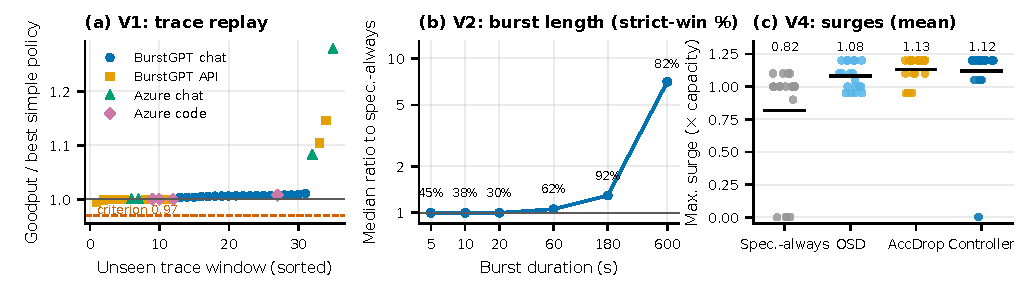
\includegraphics[width=0.58\linewidth]{figures/fig5_heldout.pdf}
\caption{Frozen-simulator validation on unseen workloads: (a) controller goodput relative to the best of five simple policies in each of \nv{v1.n} trace windows (sorted); (b) median goodput relative to \pol{SpecAlways} for bursts of a new domain, by length (labels: share of strict wins); (c) largest surge, in multiples of plain-decoding capacity, served without SLO violation in 20 scenarios (dots) and their mean (bars).}
\label{fig:heldout}
\end{figure*}

\paragraph{Unseen traffic shapes in a frozen simulator.}\label{sec:heldout} To test traffic shapes beyond the live runs, we replay traces in a fluid single-GPU simulator built from the frozen calibration file, with goodput (tokens served within the SLO) as the currency and five simple policies (\pol{NoSpec}, \pol{SpecAlways}, and \pol{OSD}, \pol{Timed}, and \pol{AccDrop}, which train on idle time, a timer, or an acceptance drop). We froze the simulator and the calibration and declared four criteria before running workloads never used in development: \nv{v1.n} unseen trace windows from BurstGPT \citep{wang2024burstgpt} and the Azure 2023 traces \citep{patel2024splitwise} at three or four load scales, 60 random bursts of a new domain, 40 Chinese regimes, and 20 surge scenarios at seven surge levels (\cref{app:sim}).

Figure~\ref{fig:heldout} reports the outcomes (\cref{tab:heldout} in \cref{app:sim}). The goodput criterion holds in all \nv{v1.n} trace windows: the controller is never more than \nv{v1.short}\% below the best simple policy and is the best policy in \nv{v1.best}. The training criterion fails in four Azure chat windows (\pol{OSD} trains on fewer tokens). Three pre-declared expectations did not survive (\cref{app:sim}): training pays back reliably only for bursts of about three minutes or longer (strict wins \nv{v2.d60.win}\% at 60\,s, \nv{v2.d180.win}\% at 180\,s), the controller's margin over \pol{SpecAlways} in the \nv{v3.n} Chinese regimes is \nv{v3.feas.min}--\nv{v3.feas.max}$\times$ rather than the pre-declared $1.5\times$, and \pol{AccDrop} tolerates surges as well as the controller; the controller's advantage lies in meeting all four criteria at once.

\subsection{Cross-engine deployment and runtime overheads}\label{sec:sglang}

\begin{table}[t]
\caption{SGLang: phase-B throughput relative to \pol{Static} (paired mean $\pm$ sd, \%; best in bold) and the worst ratio to the scenario's best policy.}
\label{tab:sgl_main}
\centering\footnotesize\setlength{\tabcolsep}{3pt}
\IfFileExists{tables/tab_sgl_main.tex}{
% SGLang results -- grouped by model architecture
\begingroup
\renewcommand{\arraystretch}{1.20}
\setlength{\tabcolsep}{3pt}

\begin{tabular}{@{}lcccc@{}}
\toprule

% ===== Model architecture groups =====
&
\multicolumn{2}{c}{
  \textbf{Qwen3-8B (Dense)}
}
&
\multicolumn{1}{c}{
  \shortstack{
    \textbf{30B-A3B}
    \textbf{(MoE)}
  }
}
& \\

\cmidrule(lr){2-3}
\cmidrule(lr){4-4}

\textbf{Policy}
& \textbf{Code}
& \textbf{Chinese}
& \textbf{Code}
& \textbf{Worst} \\

\midrule

\pol{Static}
& 10.4k tok/s
& 6.4k tok/s
& 6.8k tok/s
& 0.523 \\

\pol{Plain}
& \cellcolor{tabBest}
  $\boldsymbol{+16.0\pm0.6}$
& \cellcolor{tabBest}
  $\boldsymbol{+91.4\pm0.9}$
& $-31.9\pm0.5$
& 0.628 \\

\pol{Switch}
& $-0.5\pm0.2$
& $+37.9\pm3.9$
& $-0.7\pm0.9$
& \cellcolor{tabBest}\textbf{0.721} \\

\pol{TIDE}
& $+15.8\pm1.0$
& $+35.8\pm1.6$
& \cellcolor{tabBest}
  $\boldsymbol{+8.4\pm1.0}$
& 0.710 \\

\addlinespace[3pt]

% ===== Proposed controller =====
\rowcolor{tabFull}
\pol{Full}
& $+15.8\pm1.0$
& $+37.0\pm6.6$
& $+7.7\pm0.5$
& 0.716 \\

\bottomrule
\end{tabular}
\endgroup
}{}
\end{table}

\paragraph{A second engine.} We reimplemented the three engine extensions on SGLang 0.5.10 \citep{zheng2024sglang} as a runtime patch of its EAGLE-3 path, writing the same shared-memory records, so that the harness, controller, trainer, prompts, and seeds of the vLLM checkpoint run unchanged (\cref{app:sglang}). The port passes its checks: greedy outputs with speculation on and off agree on every prompt, toggling speculation every 0.5\,s under load completes every request with exact token counts, drafter swaps move acceptance as expected, and the exported hidden states match Hugging Face Transformers (cosine $\ge$ \nv{sgl.8b.cosmin}). After calibrating and freezing an SGLang checkpoint with the same scripts, the controller made the same decisions as on vLLM (\cref{tab:sgl_main}): on Chinese it turned speculation off and did not train; on code it trained, gaining \nv{sgl.code.full.d}\% on Qwen3-8B and \nv{sgl.moe.full.d}\% on the MoE target over \pol{Static}, where adapted drafters bring \pol{Full} level with \pol{Plain} on Qwen3-8B code and plain decoding loses \nv{sgl.moe.plain.abs}\% on MoE, as in vLLM; in every scenario it is within \nv{sgl.full_vs_loaded.maxshort}\% of the best other policy that keeps a drafter loaded. SGLang runs speculation without its overlap scheduler, so its speculation-off state is \nv{sgl.off_vs_plain.c256}\% slower than plain decoding at saturation, which leaves \pol{Plain} \nv{sgl.zh.plain_vs_full}\% ahead on Chinese (\cref{app:sglang}): a speculation switch pays fully only where the engine makes a step without speculation as cheap as plain decoding.

\paragraph{Latency and overheads.}\label{sec:overheads}\label{sec:latency} \pol{Full} changes phase-B p99 TPOT by \nv{code.full.p99}\%, \nv{zh.full.p99}\%, and \nv{moe.full.p99}\% relative to \pol{Static}; training in the SLO slack raises phase-A1 median TPOT on Qwen3-8B by \nv{code.full.a1}\% and \nv{zh.full.a1}\%, far below the SLO (\cref{app:latency}). The export path and memory reserve cost \nv{moe.infra}--\nv{code.infra}\% of phase-B throughput (\pol{Production} versus \pol{Static}), and the speculation-off state, mostly a loaded but idle drafter, \nv{zh.switch_vs_plain.abs}--\nv{code.switch_vs_plain.abs}\%, the largest overhead. No drafter swap or speculation switch caused a failed request in the \nv{n.runs} runs (\cref{app:extra}).
